\section{Connexion}

\subsection{Génération chaîne de caractère aléatoire}
    
\begin{itemize} 
\item Problématique :
Lors de la création d’un utilisateur ESTER par un autre (un médecin peut créer un compte infirmier, assistant, préventeur, et un administrateur peut tout créer), un mot de passe provisoire est communiqué à l’utilisateur pour sa première connexion.
D’autre part, le patient se connecte en utilisant un identifiant unique de 5 caractères communiqué par son médecin.
\item  Implémentation :
Pour l’implémentation, nous avons utilisé une instance de la classe SecureRandom \footnote{Cette classe fournit un générateur de nombres aléatoires (RNG) de chiffrement fort.} permettant de tirer aléatoirement les caractères de la chaîne et de la permuter aléatoirement afin d’être imprédictible.
\item  Bilan :
Le générateur de chaîne de caractères aléatoires est fonctionnel et sera utilisé pour la génération de mot de passe provisoire. Tandis que, l’identifiant du patient sera abandonné vu que la complexité de vérification de l’unicité est haute. Les M2 se chargeront de définir un algorithme générant des identifiants cryptés et uniques.

\end{itemize}

\begin{figure}[H]
    \begin{center}
	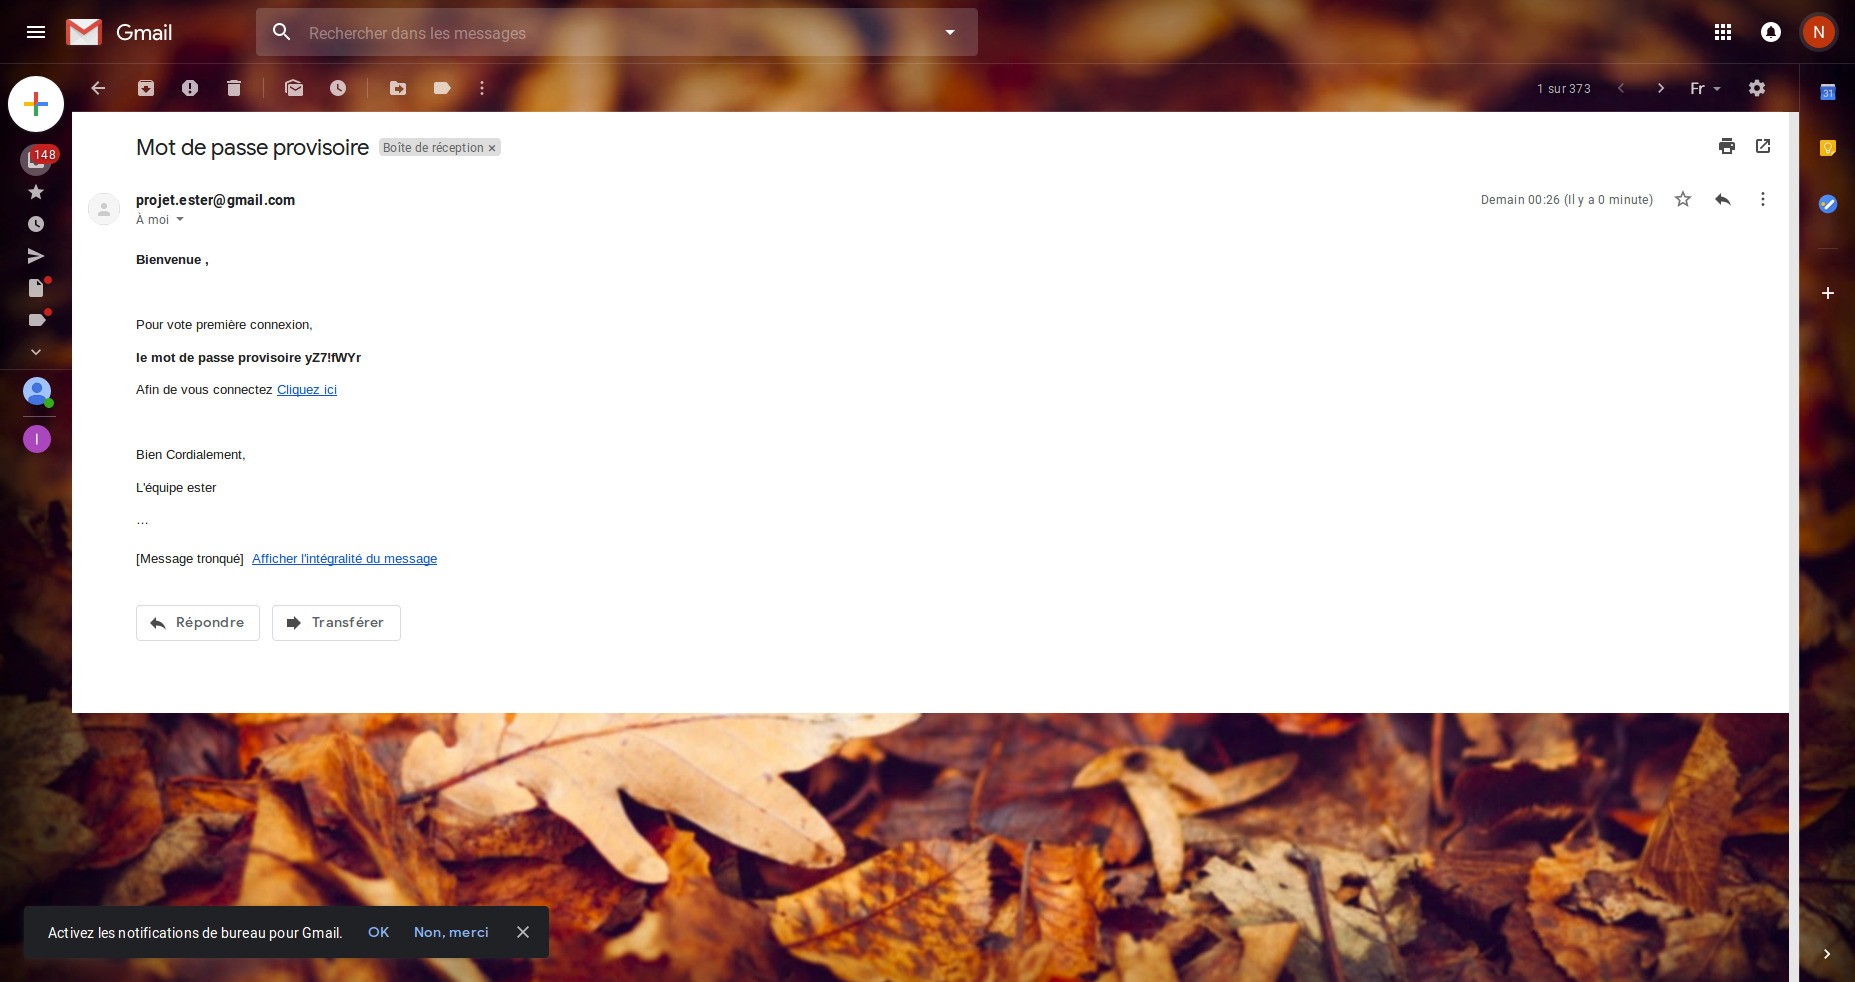
\includegraphics[scale=0.25]{img/connexion/mailCo}
    \end{center}
    \caption{E-mail pour la première connexion}
\end{figure}

\begin{figure}[H]
    \begin{center}
	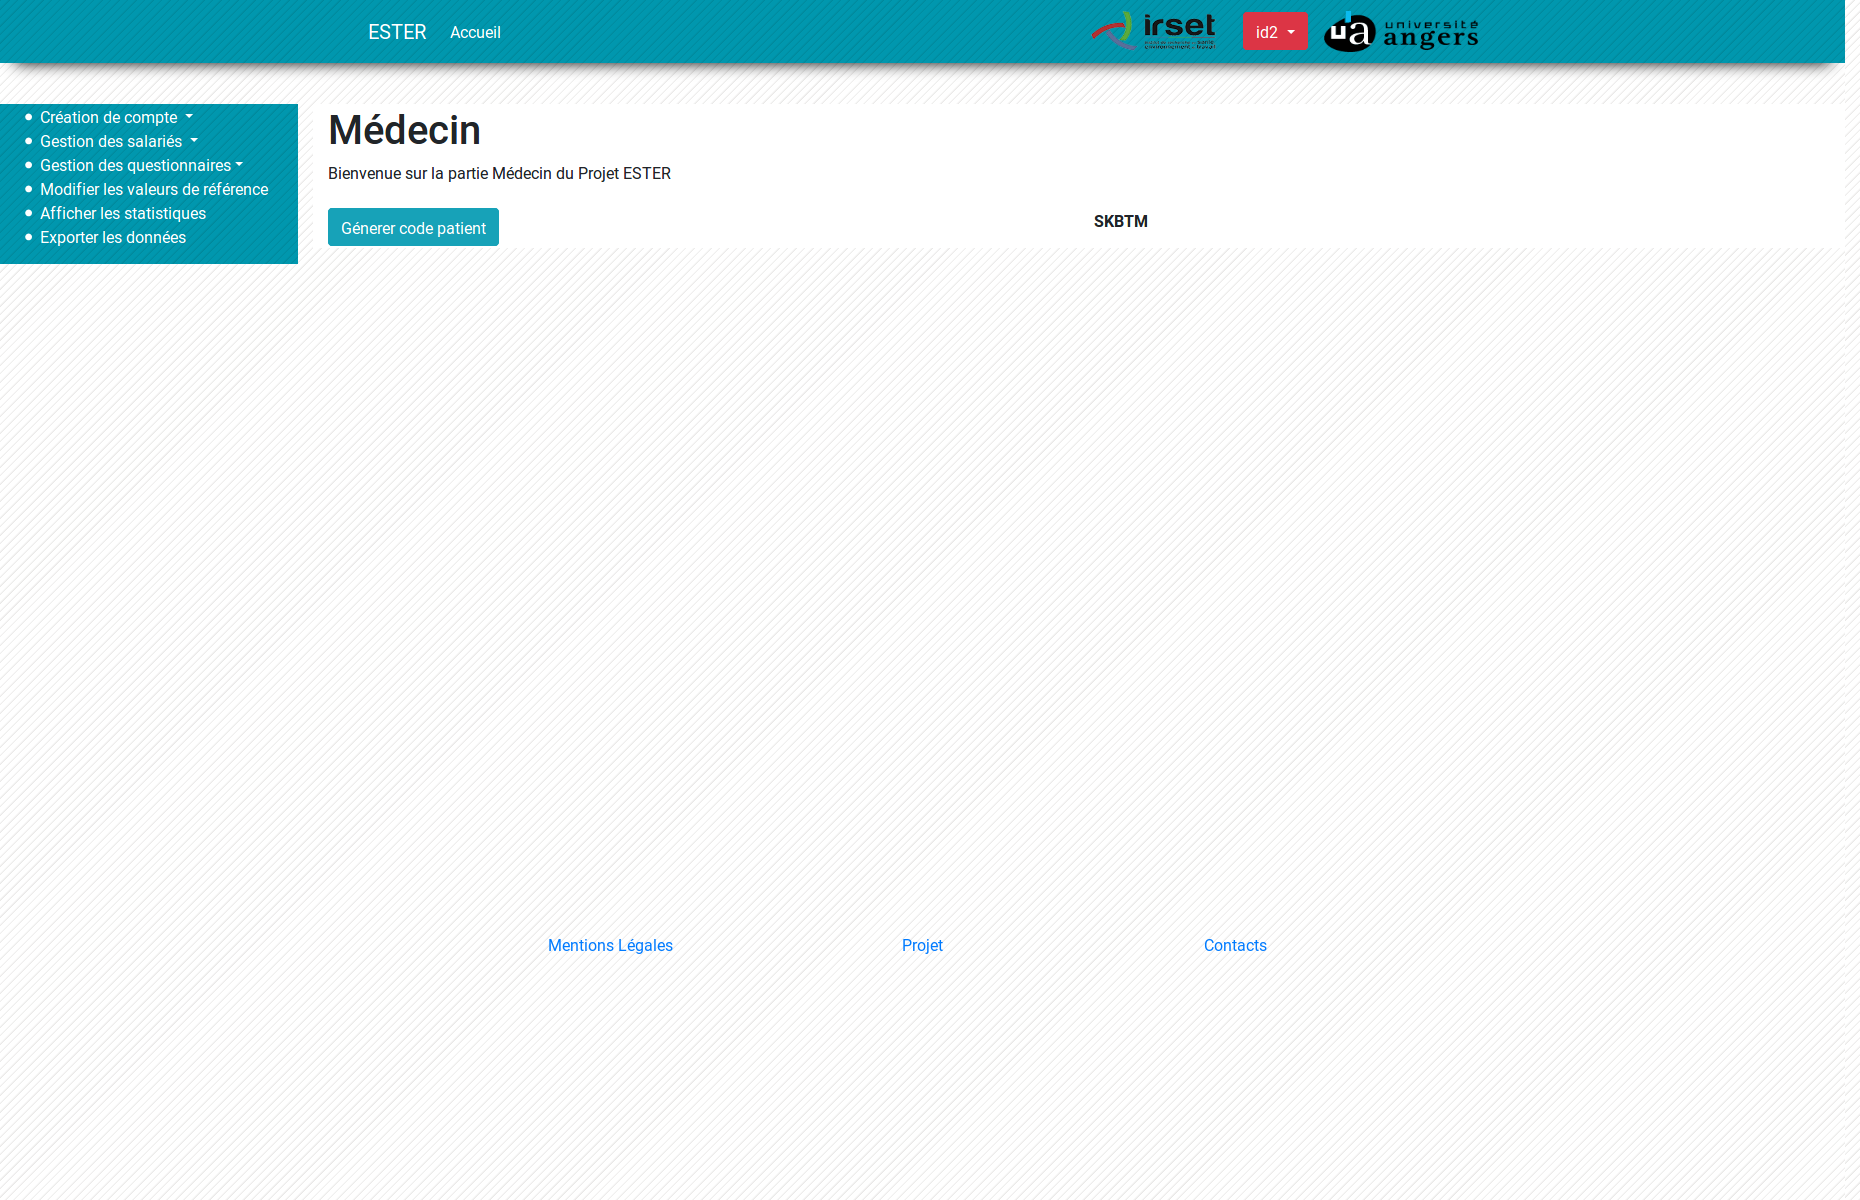
\includegraphics[scale=0.25]{img/connexion/medecin}
    \end{center}
    \caption{Générateur de codes patients}
\end{figure}

\subsection{Formulaire première connexion patient}

Lors de la création d’un compte patient seul l’identifiant est enregistré en base de données. Et afin de compléter les informations manquantes au profil à titre d'illustration: le sexe, l’âge quinquennal (pour préserver l’anonymat du patient), poste de travail, secteur d’activité et département, le patient est redirigé lors de sa première connexion vers le formulaire ci-dessous.

\begin{figure}[H]
    \begin{center}
	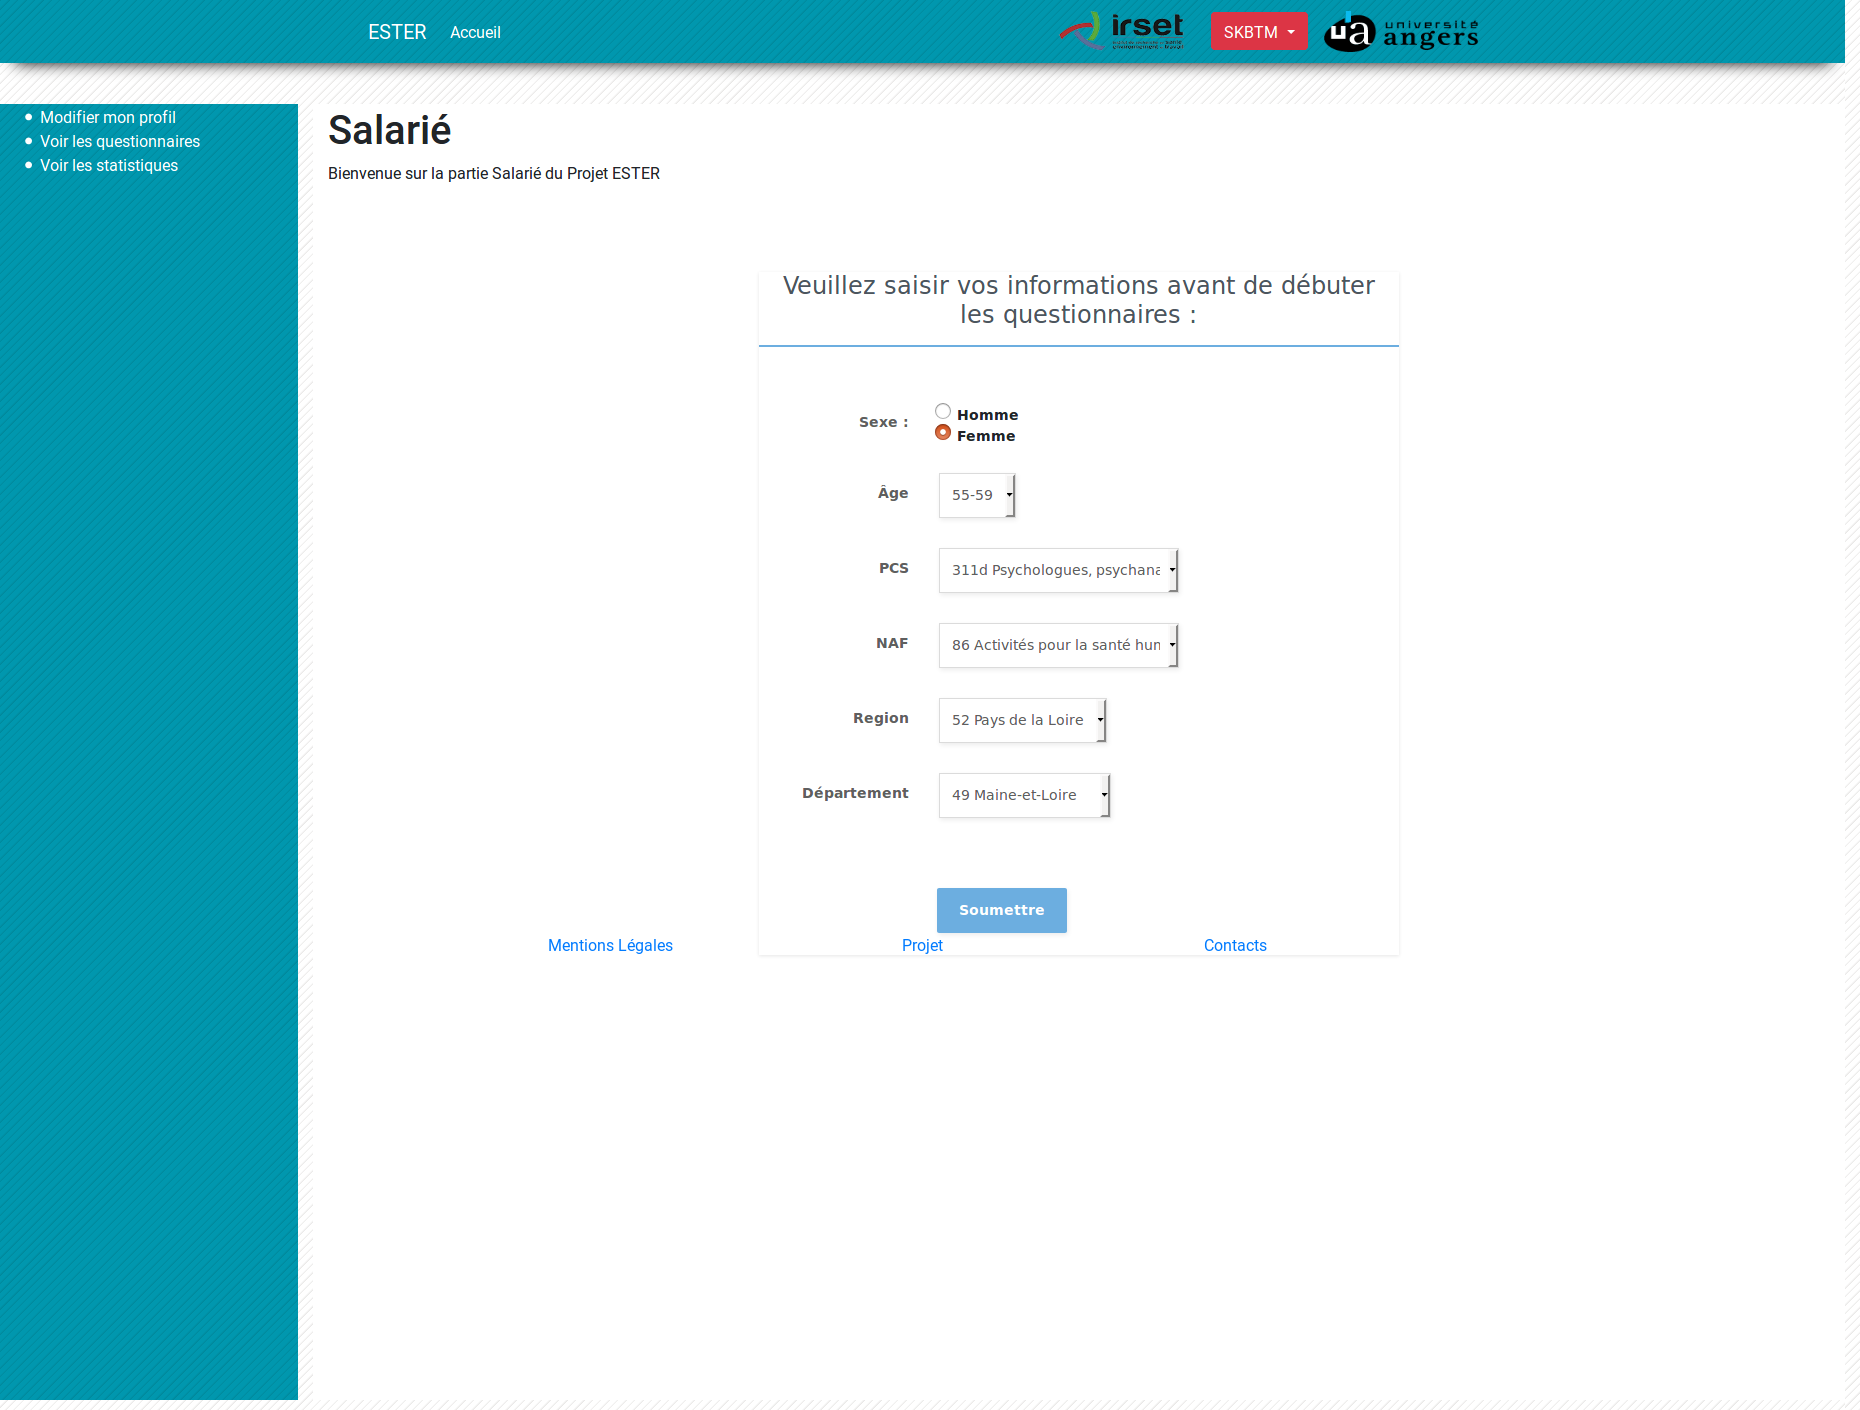
\includegraphics[scale=0.25]{img/connexion/formPatient}
    \end{center}
    \caption{Formulaire du patient à la première connexion}
\end{figure}
